\documentclass[11pt]{article}
\usepackage[margin=2cm]{geometry}
\usepackage{graphicx}
\usepackage[dvipsnames]{xcolor}
\pagenumbering{gobble}
\graphicspath{{img}}


\begin{document}

\title{ARM Checkpoint}
\author{Bartłomiej Cieślar, Jordan Hall, Ioana Mihăilescu and Oliver Killane}
\date{4 June 2021}

\maketitle

\section{Group Organisation}
    As the emulator and assembler are separate programs that can be tested and implemented independently, we have made a group decision to complete them in parallel. Although both parts are finished and the extension is currently in development stages, this report will primarily focus on the emulator.
    \begin{center}
        \begin{tabular}{ r | l }
            \textbf{Emulator} & \textbf{Assembler} \\
            Ioana \& Oliver & Bartłomiej \& Jordan \\
        \end{tabular}
    \end{center}
    \begin{center}
        \begin{tabular}{r | l}
        \textbf{Concept} & \textbf{Description} \\
            \hline 
            
            Daily Standups & Bring up any issues with each other's code, decide what to work on for the day. \\
            Status Diagram & Each function is given a rating determining progress status. (\textcolor{red}{todo}/\textcolor{orange}{implemented}/\textcolor{OliveGreen}{tested}) \\
            Merge Requests & New features are done in separate branches, then merged into \textbf{emulate} or \textbf{assemble}\\&to allow for reviews. \\
            Pair programming & Code live on call, and with VSCode LiveShare to reduce bug incidence. \\
            Unit Tests & Create unit tests for separable functions as they are being implemented. \\
        \end{tabular}
    \end{center}
    \subsection*{Development Cycle}
        \begin{center}
            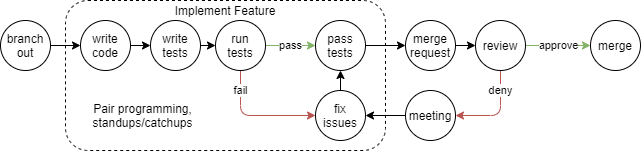
\includegraphics[width = \textwidth]{development cycle}
        \end{center}
    \subsection*{Group Function: \textcolor{OliveGreen}{excellent}}
        By splitting the project and developing for predefined interfaces, members can work at their own pace. For any given design choice, at most two members have to decide (avoiding the "too many cooks problem").
        \newline\newline
        In particular, pair programming has been very effective in writing bug-free, readable code on the first pass of our development cycle. In the extension we will continue this strategy, specifically for test creation, as faulty unit tests have been a time consuming issue. 
        \newline\newline
        Another improvement we could make is squashing commits and deleting the source branch when merging. This would improve project hygiene while preserving the commit message history and removing any "dead" branches. Furthermore, we could use more descriptive branch names to ease confusion about their contents.

\section{Implementation Strategies}
    \subsection*{Project Structure}
        \begin{center}
            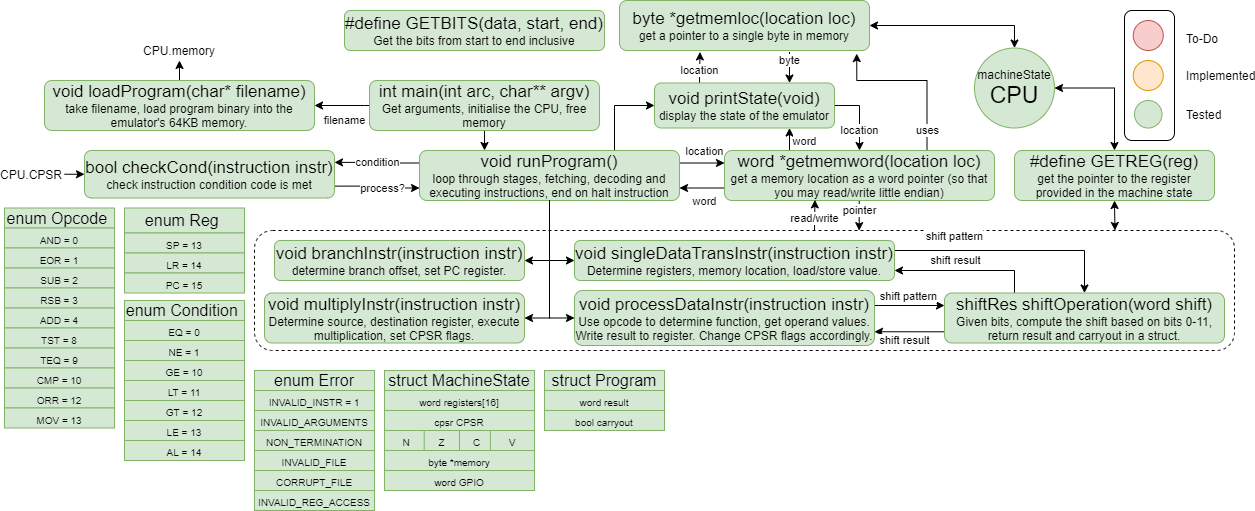
\includegraphics[width = \textwidth]{project status}
        \end{center}
    \begin{center}
        \begin{tabular}{l | l | c}
            \textbf{Step} & \textbf{Functionality} & \textbf{Subroutine} \\
            \hline
            (1) & Set the CPU up and initialize values to zero. & \textcolor{OliveGreen}{main} \\
            (2) & Write the input file to the CPU memory. & \textcolor{OliveGreen}{loadProgram}\\
            (3) & While no halt instruction has been detected and no critical error has occurred: & \textcolor{OliveGreen}{runProgram} \\
            (3a) & Read the current instruction and increment the PC.  & \textcolor{OliveGreen}{runProgram}\\
            (3b) & Determine whether instruction condition code is met by the CPU's CPSR register state. & \textcolor{OliveGreen}{checkCond}\\
            (3c) & If so, determine the instruction type.  & \textcolor{OliveGreen}{runProgram}\\
            (3d) & Send the instruction to the appropriate function to change the CPU state. & \textcolor{OliveGreen}{Instr Functions}\\
            (4) & Display the CPU state and exit. & \textcolor{OliveGreen}{printState} \\
        \end{tabular}
    \end{center}
    
    \subsection*{Notable design decisions}
        \subsubsection*{Offset to instruction fetch}
           The PC is always 8 bytes ahead of the instruction being computed. As in the pipeline, only the 'execute' stage changes the state of the CPU. We decided to avoid simulating the fetching and decoding stages directly since processing the instructions separately improves performance due to avoiding unnecessary intermediate representations of instructions. The performance gained over a more complex implementation will help with the development of the extension.
        \subsubsection*{CPSR register as separate from other registers}
            Since we only care about the CPSR register's most significant 4 bits and the register itself cannot be accessed with any instructions, we only store those bits. This allows for more readable code (access via CPU.CPSR.N/Z/C/V) and faster changing of the flags (no masks or shifting required).
        \subsubsection*{CPU global variable}
            The CPU state is held in a single global struct, which is side effected by all functions changing its state.
\end{document}

